%Intro_El_Measurment
\chapter{Introduction to Electrical Measuring Devices}
\LARGE \textbf{(Not Step-by-step, read before class)}
\normalsize
\vspace{0.25in}

Last week we tackled very simple computer control, but we said we also want
to transfer data from our experiment to our computer. In order to understand
how to do that, we need to know what things we can measure with electronic
devices. We will take on this question today, but we will get practice
making these measurements with special equipment designed just for making
these measurements. These devices won't send the data they measure to our
computers, but they will display it so we can see the data.

Once we know how to make some basic measurements with these stand-alone
instruments, then we can consider how we would make a new instrument to
measure something else. We will build a current measuring device, an \emph{
ammeter} out of electrical components and a \emph{voltmeter}. This will be
something we do over and over again. We will build a new instrument using
instruments we already know, and some electrical equipment.

This lab consists of a large pre-reading section that will give you
background information, and then at the end an assignment where I will ask
you to practice making these measurements with our equipment. Notice this is
different than last week's lab reading. Last week the reading went step by
step through the assignment. This week the assignment is at the end and you
will have to think through how to do the problems as a group.

\section{What we measure: Voltage (and Current)\label{Voltage Measurement
with Meter}}

The two easiest electrical measurements to make are voltage and current
measurements. So physicists try to turn all other types of measurements into
voltage or current measurements. You may want to measure relative humidity.
But to record relative humidity on our computer we need to convert relative
humidity into a voltage or current! We will do experiments that do this type
of conversion, but first, let's learn about voltage and current so we can
see how electronic systems measure them.

Voltage is really ``electrical potential
difference,'' which is the difference between electrical
potential energy per unit charge at two different circuit locations. Last
lab we said voltage was a comparison, and this is the comparison. We compare
the potential energy at two different circuit locations, only we divide the
potential energy by the charge of an electron.

To get a feel for how this works, think of a change in gravitational
potential energy, $\Delta U_{g}$. If we wanted to measure the difference in
potential energy between the top of a hill and the bottom of a hill, we
would need to place some sort of device both at the top and at the bottom of
the hill. 
\begin{figure}[h!]
	\centering
	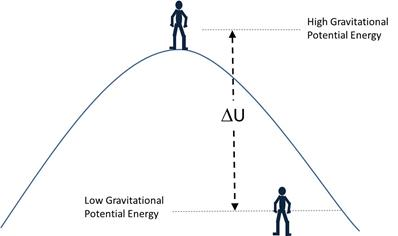
\includegraphics[width=3.3537in,height=1.9977in]{PH4CAU0F}
\end{figure}

We have to do the same thing in
our electrical case. We need two ``probes,'' one placed at the high potential and one placed
at the low potential. For example, we could have the circuit that you see in the next figure.

\begin{figure}[h!]
	\centering
	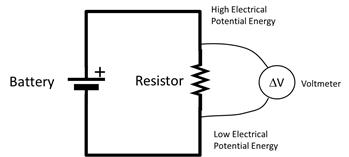
\includegraphics[width=2.9438in,height=1.3353in]{PH4CAU0G}
\end{figure}

The positive end of the battery is like the top of the hill. It provides a high electrical potential energy. So we put one probe at the top of the ``hill'' or the plus side of the battery, and the other on the bottom of the ``hill'' or minus side of the battery. The negative side of the battery provides a low electrical potential energy. With this we measure how high our potential
``hill'' is. The difference between these two measurements is called \emph{voltage.} You should ask yourself
``what would happen if you got the probes
backward?''

In the next figure you can see how to actually perform this voltage measurement with one of our meters.

\begin{figure}[h!]
	\centering
    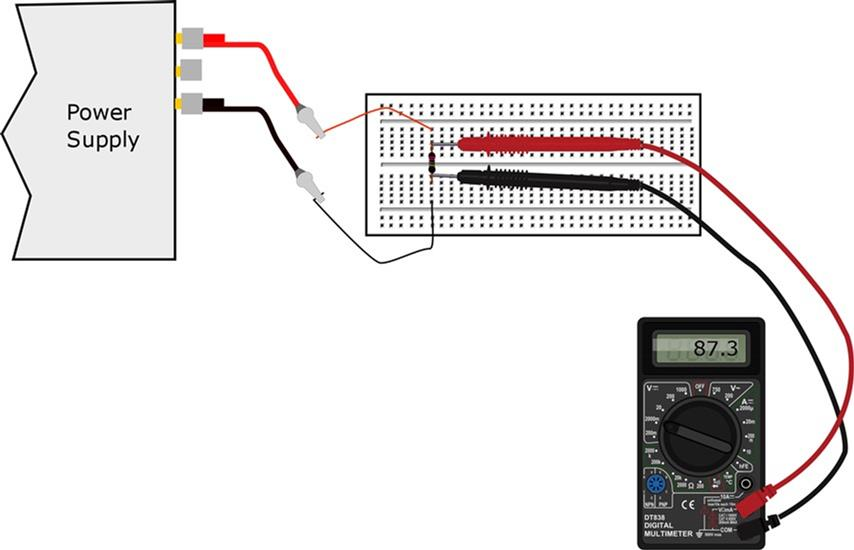
\includegraphics[width=5.5997in,height=3.614in]{PH4CAU0H}
\end{figure}

We say we measure voltage ``across'' a circuit element. This makes some sense if you consider that we very seldom stand batteries up so their electric potential is greater in the same direction as their gravitational potential. Batteries, resisters, capacitors, etc, often lie down, and we measure ``across'' them by putting the positive probe on the high potential side and the negative probe on the low potential side. Even though the battery is lying down, we are still measuring a higher and lower potential energy difference. Knowing a little about voltage, let's look at our devices that produce voltages and then the devices that measure voltages.

\section{Stand-Alone Experimental Hardware}

In today's lab we will study four hardware devices. It might be better to skim this part before lab, then read it in detail with your lab group in class when you have the equipment in front of you. \textbf{But do read these sections!} You can damage your equipment if you don't know how the equipment works. So read these sections as you work! And you need to read the sections about  designing new measuring devices below (starting in section \ref*{New_Instrument_Section}), so skim the equipment sections, but not the rest!

Here is a list of the devices we will study in this time's lab:
\begin{enumerate} 
	\item a power supply
	\item a signal generator
	\item a multimeter
	\item an oscilloscope.
\end{enumerate}

We will call these ``stand alone'' instruments because they are independent boxes that do their job of measuring or generating signals without a computer connected to them. The power supply and the signal generator make voltage signals. The other two devices measure them. Let's look at the power supply and signal generator first, then take on the measuring devices.

\subsection{Power Supply}

A power supply is like an adjustable battery. Batteries have fixed voltages. But a power supply may have an adjustable voltage. 

\begin{figure}[h!]
	\centering
	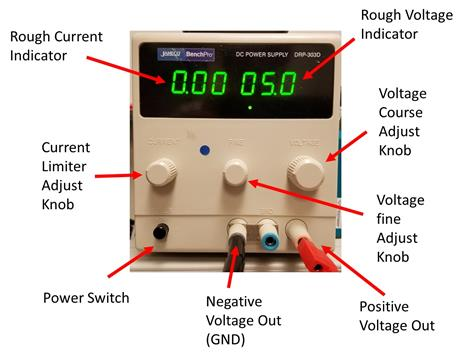
\includegraphics[width=3.9237in,height=%
3.0191in]{PH4CAU0I}
\end{figure}

Usually a power supply takes electrical energy from the wall outlets and converts that energy into the specific voltage that we want for our experiment. So it is like a battery, but must be plugged into the wall. Our power supplies are designed to keep us safe. They are current limited, meaning that they try not to give too much charge flowing through our wires. Sometimes this is a problem
because they are too limited. There is a current limiting knob that you can turn to allow a little more current. Be careful when you use this. The voltage may jump wildly when you turn the current knob! It is best to turn all the knobs down as low as they will go before you turn on the power
supply. Then, after turning on the power supply, increase the current knob about half a turn and then slowly turn the voltage knob up to your desired voltage. If the voltage stops increasing, turn the voltage knob back down a bit, and turn up your current limiter knob some more. Then try your voltage knob again.

Some of our electrical devices are quite delicate, and will literally burn up if you apply too much current or voltage. In today's lab, we will practice using our power supply so we are prepared when the delicate components come out later.

\subsection{Signal Generator}

\begin{figure}[h!]
	\centering
	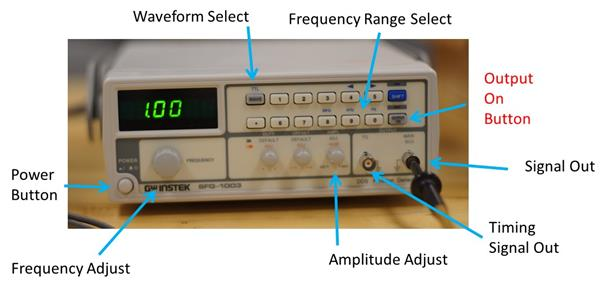
\includegraphics[width=5.093in,height=3.0in]{PH4CAU0J}
\end{figure}

The signal generator is a fancy power supply. It makes changing voltages. It can make voltages in sine, square, and triangle patterns. These time-varying signals have a maximum voltage (called the amplitude) . We will use both the wave output and a timing signal that the wave generator creates. Each has their own Bayonet Neill--Concelman connector (usually just called a BNC connector) on the
front of the signal generator. You will need a cable with BNC connectors on one end (and maybe alligator clips on the other end) to use this device. There is an amplitude knob on the front of the signal generator. Because the signal generator makes a voltage that changes in time, the amplitude of the signal must be in voltage units. We should be careful not to set the signal amplitude (voltage) too high or we run the risk of destroying our measuring devices. Again turn the amplitude (voltage) down before you connect the box to our electrical components. Then turn up the voltage to what you want in a safe way.

There are frequency range buttons (using the shift button) near the middle of the device panel. To change the frequency, you use the shift and range buttons to set which digit you are adjusting, then turn the frequency knob to make the change. An annoying feature of our frequency generators is that you must push the ``output on'' button or they don't output a signal. When everything is set up right, we get a sine wave (or square wave, or triangle wave) out. Here is a signal from the signal generator displayed on one of our measuring devices, the
oscilloscope. 

\begin{figure}[h!]
    \centering
    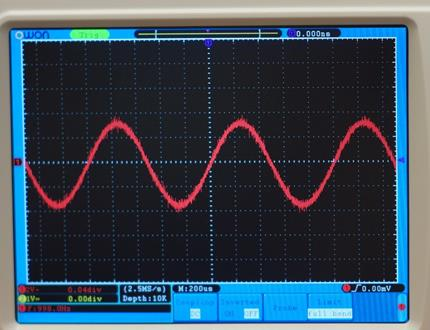
\includegraphics[width=3.0in,height=2.0in]{PH4CAU0K}
\end{figure}

Of course, simple batteries are sources of voltage, and so are many other things.

\subsection{Voltmeter}

Our first measurement device is voltmeter. It measures the electric potential (voltage) between its two leads (sometimes called ``probes'' ). Here is a picture of one of our multi-meters set to measure voltage.

\begin{figure}[h!]
	\centering
	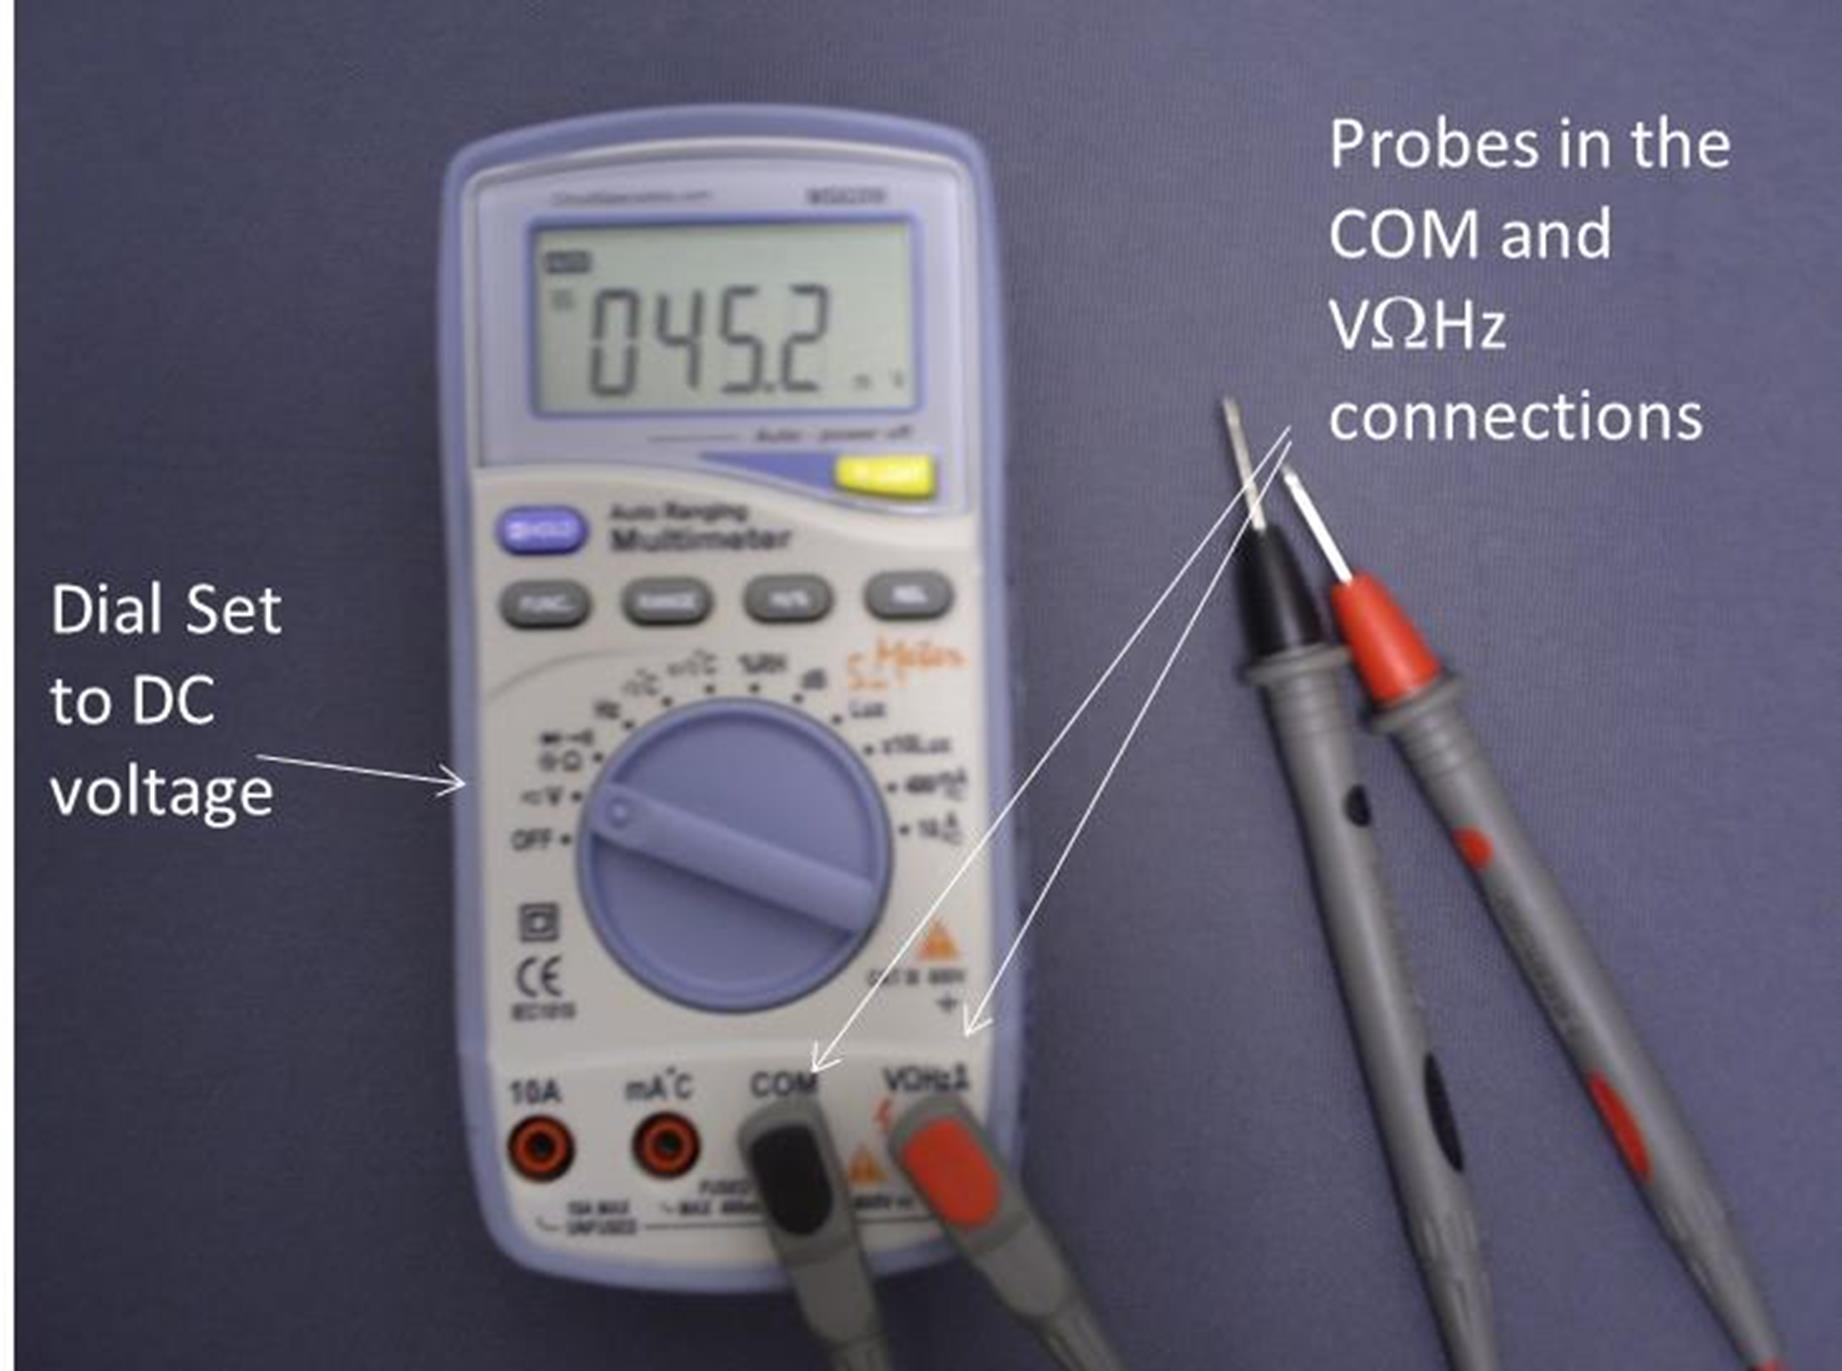
\includegraphics[width=3.116in,height=2.3266in]{PH4CAU0L}
\end{figure}

The display is set to read voltage by turning the dial to the $\unit{V}$ position. There are often two voltage settings. The one that has a wavy line next to it is alternating voltage. The one that has a straight line with three dots under it is the direct current (DC) voltage. These words might not mean much to you yet if you are just starting PH220. So for now, we will just use the DC voltage setting. As you learn more, we may use the alternating voltage setting. The leads (probes) should be connected to the COM (common) and $\unit{V}\unit{\Omega}\unit{Hz}$ connectors. Note that connecting your probe leads to the wrong position can blow the fuse (or worse) in your meter and make subsequent readings very wrong. You should make sure you don't do this, and watch to make sure someone else has not done this before you. If the meter seems crazy, it just may be. We have several different voltmeter models. Here is a picture of a different model.

\begin{figure}[h!]
   \centering
   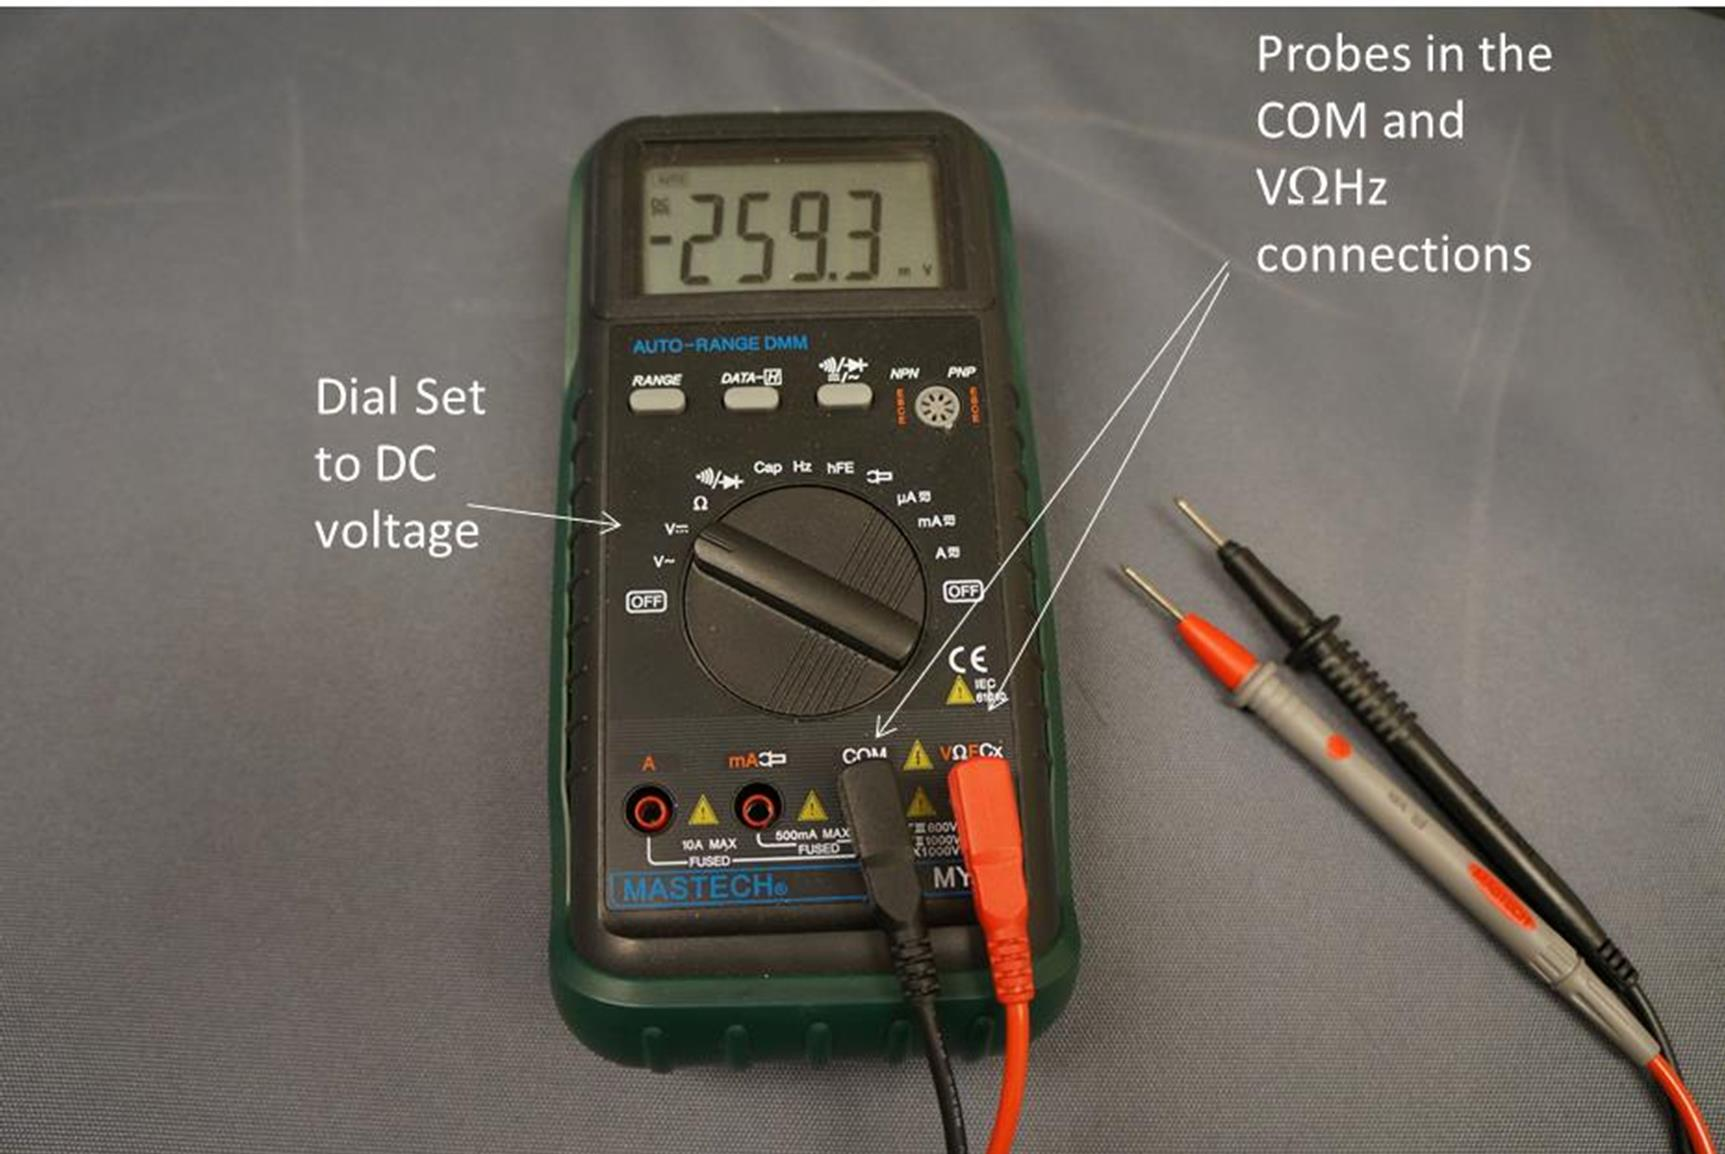
\includegraphics[width=2.9199in,height=1.962in]{PH4CAU0M}
\end{figure}

You will notice that there are other settings besides volts. Our meters are all multi-meters. That means that they can measure more than one thing. We will use several of the settings throughout the semester.

\subsection{Oscilloscope}

Our next device, the oscilloscope, is just a fancy voltmeter. Unlike the multimeter, it usually just measures voltage. But it does it with flare!

The oscilloscope can measure changing voltages very accurately and usually has a way to graph the changing voltage. The standard is a voltage vs. time graph. A sinusoidally varying voltage should look something like this when plotted. 

\begin{figure}[h!]
	\centering
    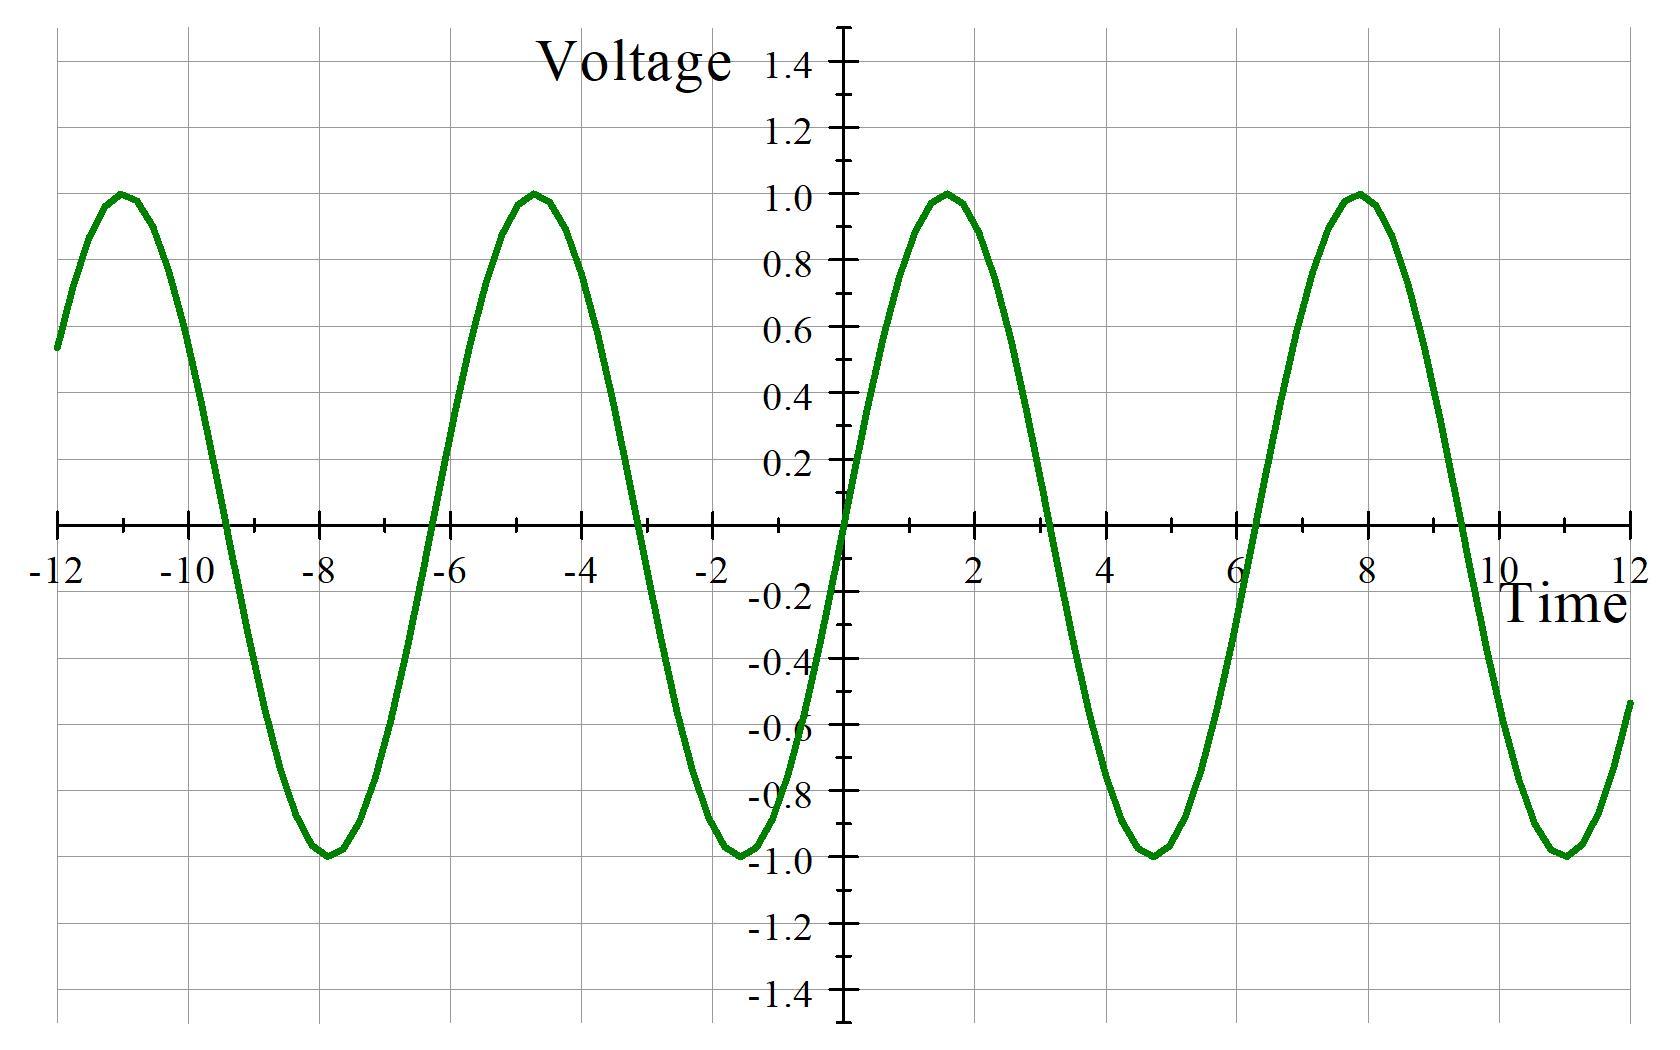
\includegraphics[width=3.00in,height=2in]{PH4CAU0N}
\end{figure}

And that is what our oscilloscope does. We should see something like this on the oscilloscope screen. From our discussion of the signal generator, you know that this is just what we see.

\begin{figure}[h!]
	\centering
    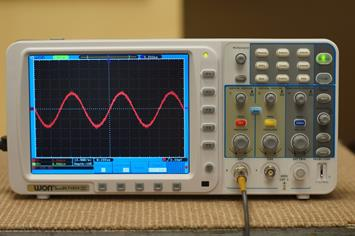
\includegraphics[width=3.00in,height=2.00in]{PH4CAU0O}
\end{figure}

If the changing voltage is periodic, the oscilloscope has a way to use this fact to stabilize the graph so you can see the details more clearly. This stabilization is called ``triggering'' and
on our oscilloscopes there are buttons and knobs on the right hand side of the oscilloscope that adjust the triggering to make the graph more stable (or less stable). The photograph of the sine wave above was taken by stabilizing a sine wave from our signal generator. The oscilloscope starts
plotting at the same part of the wave each time, so the periodic signal seems to stand still. To do this we must ``trigger'' the graph at some good starting point. Our oscilloscopes have a build-in circuit that can watch for the same part of a signal and start the graph in the same place each time. One of the knobs adjusts the trigger point. 

\begin{figure}[h!]
	\centering
    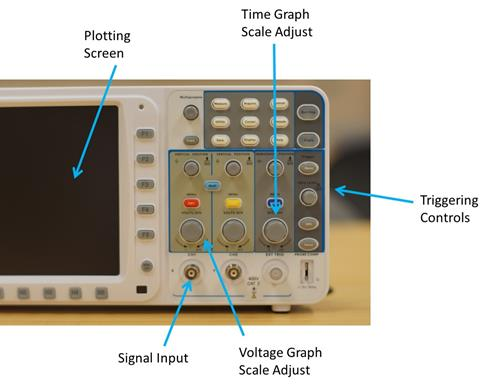
\includegraphics[width=4.00in,height=3.00in]{PH4CAU0P}
\end{figure}

The other controls adjust the horizontal and vertical axes. The vertical axis is voltage, and the voltage axis control is next to the signal input toward the bottom middle of the front panel. To the right of this is the horizontal axis control, which is time. You can choose how many volts per division with one knob and how many seconds (or fractions of seconds) per division you have on your graph with another knob. In the next figure you can see a signal on the oscilloscope screen. 

\begin{figure}[h!]
	\centering
	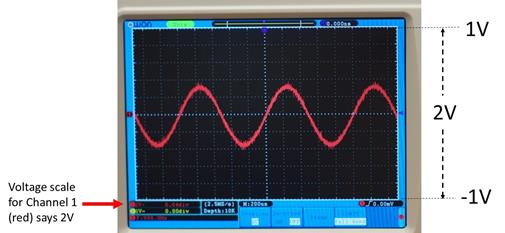
\includegraphics[width=4.2505in,height=1.9718in]{PH4CAU0Q}
\end{figure}

In the bottom left-hand corner there is a red dot and a voltage given. This is the voltage displayed across the whole screen. Since when this photo was take the voltage knob was set to 
$2\unit{V}$, this means that the bottom of the screen represents $-1\unit{V}$ and the top of the screen represents $+1\unit{V}.$ 

\begin{figure}[h!]
	\centering
	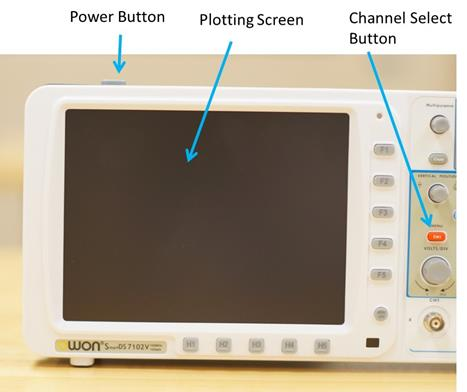
\includegraphics[width=3.9364in,height=3.3076in]{PH4CAU0R}
\end{figure}

There are two signal inputs because our oscilloscopes can look at two different voltage signals at the same time. Each signal input is called a ``channel.'' Each channel has it's own voltage scale knob and voltage scale indicator in the bottom left-hand corner. They share the same time scale.

The channel inputs each have a BNC connector. We use oscilloscope probes connected to these connectors. Notice that since there are two channels, an oscilloscope can measure two voltages at once. But that means we may need two probes!

To check that our oscilloscope is working correctly we can measure a known voltage, say, the voltage of a regular battery.

\begin{figure}[h!]
	\centering
	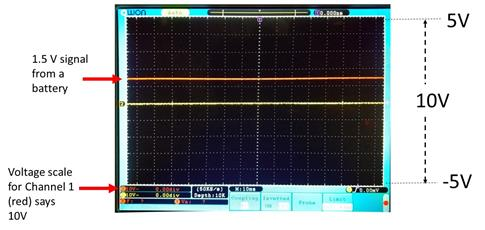
\includegraphics[width=4.0836in,height=1.9458in]{PH4CAU0S}
\end{figure}

Notice that I changed the voltage scale knob position so that now the oscilloscope screen has a $10\unit{V}$ total potential change. That means that we have $5\unit{V}$ at the top of the screen and $-5\unit{V}$ at the bottom of the screen. The screen is divided into little boxes. There are five rows of boxes from the bottom to the top of the screen. Each box represents $1/10$ of the total voltage. Since we have $\Delta V=10\unit{V},$ each box represents $\Delta V=1\unit{V}. $ So our battery voltage should give us one and a half boxes. And that is just what we got.

But sometimes the oscilloscope does not get the right voltage. If this happens we need to calibrate the oscilloscope. Every time we use an Oscilloscope it is a good idea to check it to make sure it working well. Our oscilloscopes have a test voltage to use just for this purpose.

\begin{figure}[h!]
    \centering
    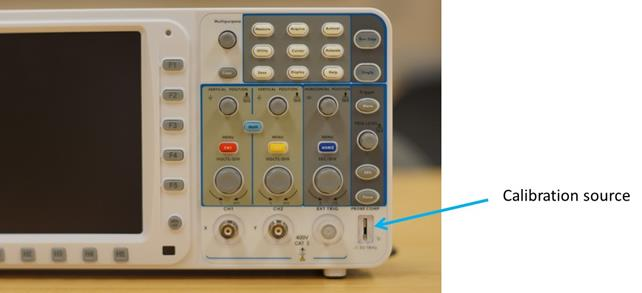
\includegraphics[width=3.70in,height=1.50in]{PH4CAU0T}
\end{figure}

The calibration source makes a $5\unit{V}$ square wave (try it to see what that looks like!). If we use this calibration source we should get something like what you see in the next figure. 

\begin{figure}[h!]
	\centering
    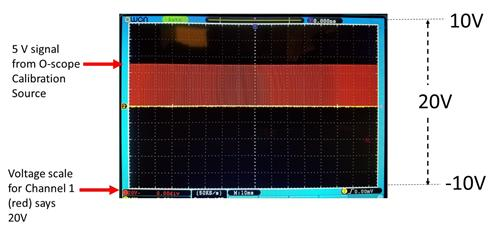
\includegraphics[width=4.00in,height=2.00in]{PH4CAU0U}
\end{figure}

If you don't get $5\unit{V},$ then some thing is wrong and you will need to go through the oscilloscope's calibration procedure. That is in the oscilloscope manual and you can find
the manual on-line.

\section{Current}

Our multimeters have a current setting as well as a voltage setting. Current is a flow of charge. This is like a water current, which is a flow of water. Only we have a different thing flowing. We have a flow of charge. In the wires in our Arduino, the moving charged things are (mostly) electrons. We can write the flow of something as 

\begin{equation*}
	I=\frac{\Delta Q}{\Delta t}
\end{equation*}

where for us $\Delta Q$ is the amount of charge that has gone by in the time 
$\Delta t.$ Physicists use the letter $I$ for electrical current.

We should take a minute to think about what to expect when we allow charge to flow. Think of a garden hose. If the hose is full of water, then when we open the faucet, water immediately comes out. The water that leaves the faucet is far from the open end of the hose, though. We have to wait for it to travel the entire length of the hose. But we get water out of the hose immediately! Why? 

\begin{figure}[h!]
	\centering
    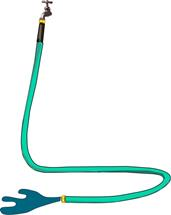
\includegraphics[width=1.4547in,height=1.8228in]{PH4CAU0V}
\end{figure}

The new water coming in causes a pressure change that is transmitted through the hose. The water at the open end is pushed out. You can tell this is the case because the water immediately leaving the hose is warm and tastes like plastic hose. After a while, the water is colder and cleaner.

Current is a little bit like this. When we flip a light switch, the electrons near the switch start to flow. But there are already free electrons in the wire. These experience a push that makes the light turn on almost instantly. But the electrons that turn on the light are not the ones
that just went through the switch. 

\subsection{Measuring Current}

Because current is a flow, to measure current we must put a meter into that flow. In a house, if you want to measure how much water is used, you connect the pipe from the city water system to a meter and then connect the meter to your house. The water flows through the meter and then goes into the pipe that brings water to the house. That way, the meter can't miss any of the water (and the city can't miss any of your payment!). The same is true for electrical current. To measure electrical current, we need to remove part of our circuit, and replace it with the meter to force the flow of electrical current to go through the meter. A schematic diagram of this might look like this: 

\begin{figure}[h!]
	\centering
    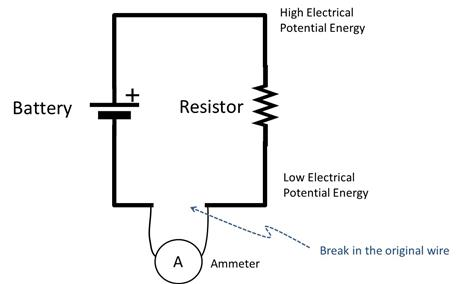
\includegraphics[width=3.8484in,height=2.3981in]{PH4CAU0W}
\end{figure}

In this diagram, you can see that the electric current must go through the current meter. In fact, it couldn't go anywhere else because part of the original circuit wire is missing. This is just what we want. To actually perform this measurement with one of our multimeters you could set up a circuit like the one in the following figure. 

\begin{figure}[h!]
	\centering
    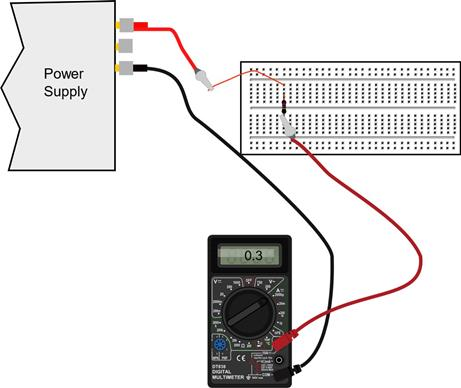
\includegraphics[width=3.8821in,height=3.2707in]{PH4CAU0X}
\end{figure}

There is one more important thing to do to make this work. We need to change the meter settings. And there are two separate changes. The first is to switch the probe connections. One probe stays in the COM or common connector, but the other needs to move to the connector marked with an ``A.'' Here is an example showing the changes with two kinds of multimeters. 

\begin{figure}[h!]
    \centering
    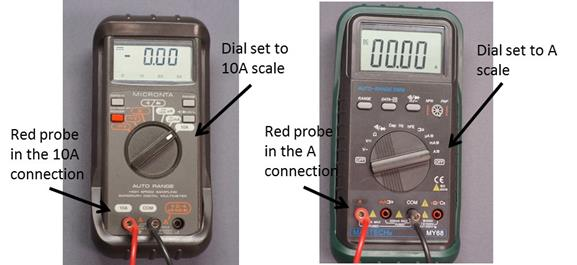
\includegraphics[width=4.858in,height=2.2423in]{PH4CAU0Y}
\end{figure}

The ``A'' stands for the standard unit of electrical current, the Ampere or Amp. With the multimeter set up like this we would call it an \emph{ammeter}. Ammeters measure electrical current.

\section{Building a New Instrument} \label{New_Instrument_Section}

We said before that physicists like to change any measurement they can into a voltage measurement. That is because we have devices like our Arduino boards that measure voltage. We build new instruments by finding ways to turn the measurement that we want to make into a voltage.

In order to build a new instrument, we need to understand the quantity that we really want to measure. We will need to understand the physics of the quantity to make a good new instrument design. Let's take an example. Suppose we wish to measure current, but suppose we don't have a current setting on our Arduino (because we don't). Could we still make a current measurement?

The secret of instrument design is to understand the physics of the measurement we want to make (current) and then see if we can turn that measurement into a voltage.

\subsection{Start with the Physics:}

Let's keep thinking of current like water in a hose. Will there be any friction associated with the water traveling through the hose? Of course there will! We usually call friction in fluids \emph{viscosity}. But it is a form of friction, and we can use our PH121 intuition about friction to see how it would work. Think of having two hoses, one twice as long as the other. Which would you expect to have more friction? 

\begin{figure}[h!]
	\centering
    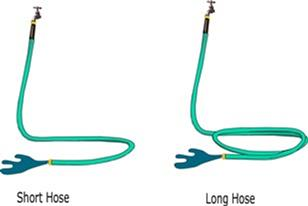
\includegraphics[width=2.6033in,height=1.7474in]{PH4CAU0Z}
\end{figure}

Our friction experience says that the longer the path, the more the friction. The current has longer to interact with the hose, so it experiences more friction. Electrical currents are like this. Longer wires give more friction.

George Simon Ohm noticed that with long metal wires, there seemed to be a linear relationship between the potential difference (voltage), the current, and the length of the wire. The longer the wire, the less the current. His work was confirmed and expanded on by others, who found that not only length mattered, but also the diameter of the wire mattered. The relationship is now expressed as

\begin{equation*}
	\Delta V=IR
\end{equation*}

$\Delta V$ is our old friend, voltage, and we know $I$ is the symbol for current, and $R$ is the slope of the $\Delta V$ vs. $I$ curve. The experiments showed this constant $R$ depended on the material. It is like our viscosity in hoses. It is the friction. The more the friction, the harder it is to get the current through the wire. But like we don't call viscosity ``friction,'' we also don't use the word ``friction'' for this friction-like term. We call it \emph{resistance.} We could solve for this resistance 

\begin{equation*}
	R=\frac{\Delta V}{I}
\end{equation*}

or we could plot $\Delta V$ vs. $I$ and the slope of this line would be the resistance.

\begin{figure}[h!]
	\centering
	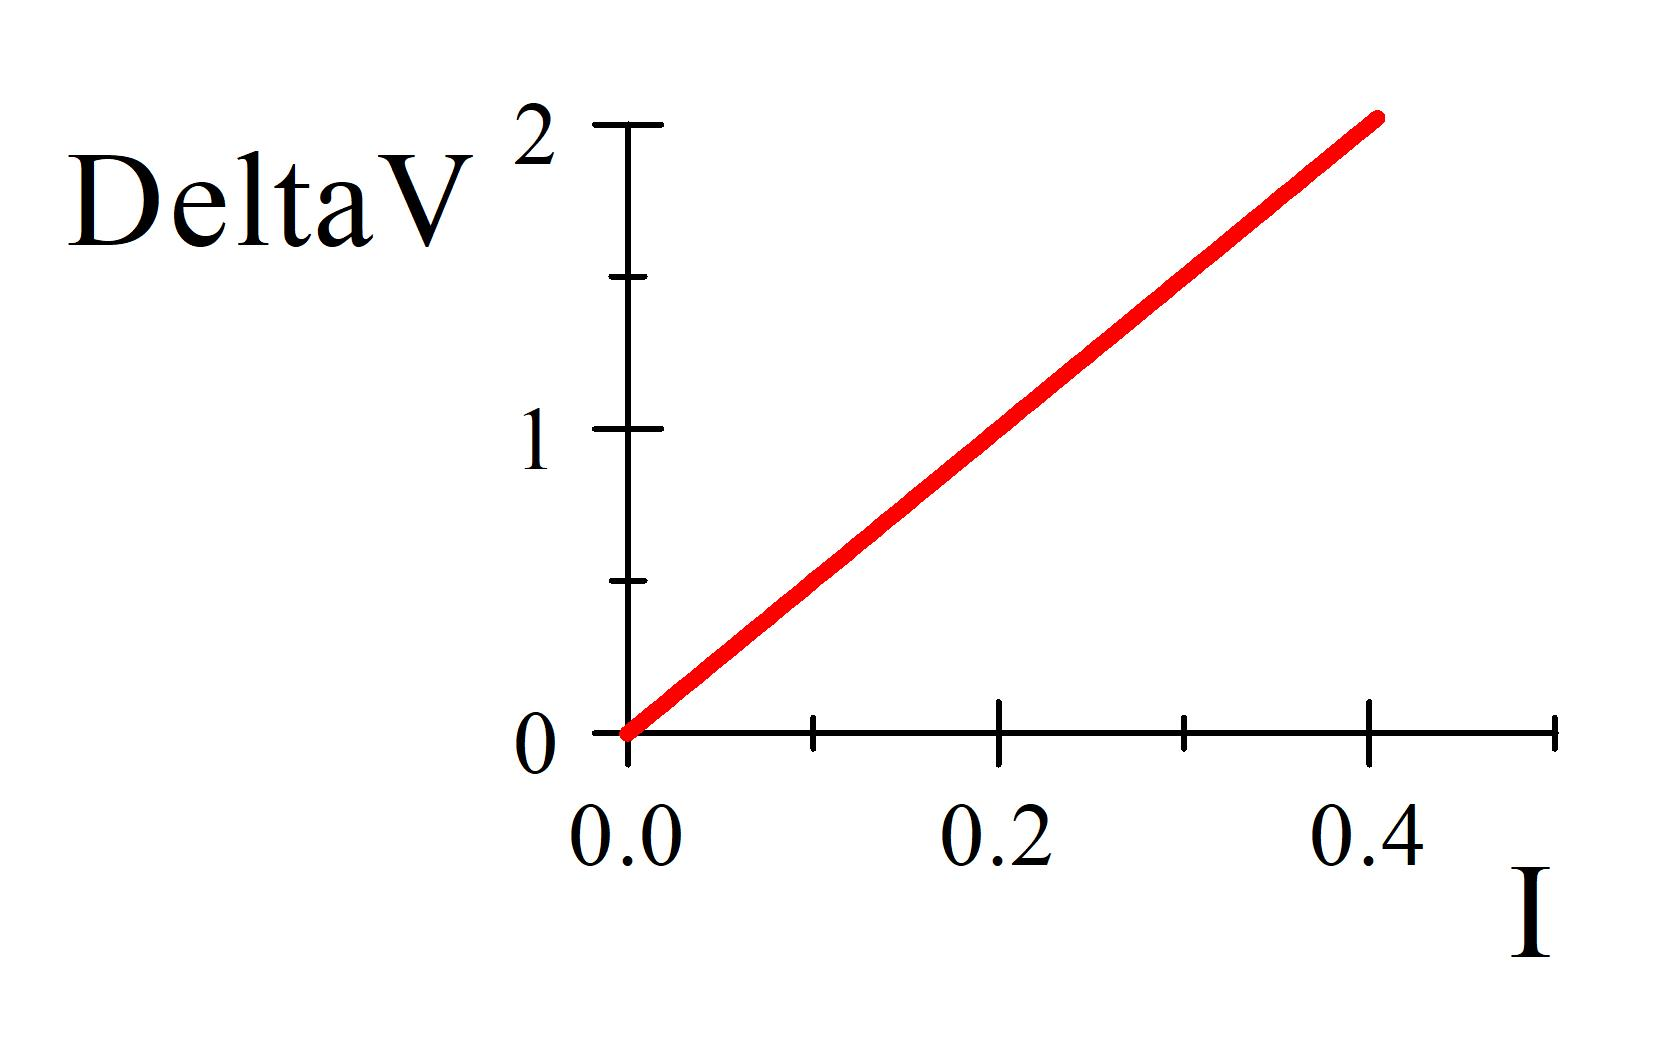
\includegraphics[width=1.9899in,height=1.3214in]{PH4CAU10}
\end{figure}

Either way, this relationship tells us that it takes more potential energy to get the same current if there is more resistance.

This is called \emph{Ohm's law.} The relationship holds well for metals and many materials, but, like Hook's law, this ``law'' does not always hold. Devices that do provide a constant resistance coefficient, $R,$ are called \emph{resisters.} We will use this symbol

\begin{figure}[h!]
	\centering
    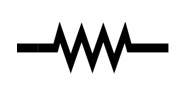
\includegraphics[width=1.742in,height=0.2794in]{Resister_symbol0}
\end{figure}

for resistors, but they often look more like this

\begin{figure}[h!]
	\centering
    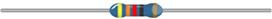
\includegraphics[width=2.2987in,height=0.179in]{PH4CAU11}
\end{figure}

Notice that this is important! We have found a way to relate our new quantity that we want to measure, current, to a voltage. We know how to measure a voltage! Our Ohm's law equation even tells us what extra part we need to convert our voltmeter into a current measuring instrument. We will need a resistor.

\subsubsection{Resistor Code}

Let's pause in our new instrument design for a moment and ask, ``how would you know the resistance of a resistor?'' Our multimeters have a resistance measuring setting, so you could measure the resistance directly using the meter. But many commercially produced resistors come conveniently marked with a color code that helps you identify their resistance. The basics of the color code are given in the following figure\bigskip 

\begin{figure}[h!]
	\centering
    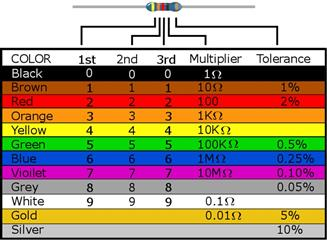
\includegraphics[width=3.2958in,height=2.4249in]{PH4CAU12}
\end{figure}

To use the code:

\begin{enumerate}
    \item Find the tolerance code band. This band is usually brown in our kit resistors and often is set off from the others a little more.

    \item Read the first color band from the side opposite the tolerance band. This will be the first digit of your resistance. I\ think the example resister on the chart has a yellow first color band, so the first digit of our resistance is $4.$

    \item Read the second color band. This will be the second digit of your resistance. I\ think the second band of our example resistor is orange, so the second digit would be a $3,$ making our resistance so far $43$

    \item Read the third color band. This will be the third digit of your resistance. I\ think the second band of our example resistor is red, so the second digit would be a $2,$ making our resistance so far $432$

    \item Read the forth color band. This is a multiplier. You multiply the first three digits by this amount. For our example resistance, I think the third band is black. Then we multiply $432$ by $1\unit{\Omega}$ to get $432\unit{\Omega}.$ This is our resistance.

    \item The tolerance band gives the uncertainty in this value. Our example resistor seems to have a brown tolerance band, which tells us our value is good to $\pm 1\%.$ For our example resistance, $1\%$ would be $0.01\times 432\unit{\Omega}=\allowbreak 4.\,\allowbreak 32\unit{\Omega},$ so our resistance is $\left( 432\pm 4\unit{\Omega}\right) .$
\end{enumerate}

We won't memorize the resistor code, but you should be able to find a resistance using the code.

If you are in doubt about what color you see on a resistor, our multimeters can measure resistance directly. 

\begin{figure}[h!]
	\centering
    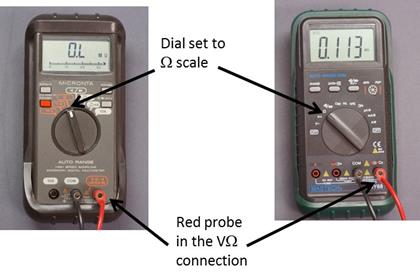
\includegraphics[width=3.5426in,height=2.3594in]{PH4CAU13}
\end{figure}

Place the red probe in the connector with a $\Omega $ marked on it and turn the dial to the $\Omega$ setting. Place the probes on either side of the resistance to be measured. Be careful/ You are a resistor too. If you touch your hands to the probes (common mistake while you try to hold the resistor on the probe ends) you may measure your resistance instead of the resistor's! You have a resistance of around half a megaohm. This is a general concern, every time you measure resistance with a meter you need to take the circuit element (resistor, light bulb, whatever) out of the circuit and measure it on it's own. Otherwise, you might be measuring the resistance of the rest of the circuit. Alligator clips are useful for this.

\subsubsection{Direction of current flow}

If you are half way through PH220 when you take this lab you will already know about current direction and can skip this section. \textbf{But if you are at the beginning of PH220, read on!} There is a historical oddity with current flow. That is that the current direction is the direction positive charges would flow. This may seem strange, since in good conductors electrons are doing the flowing and they are negative! The electrons go the opposite way the current goes. 

\begin{figure}[h!]
	\centering
     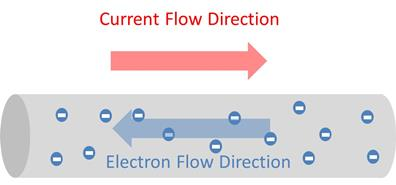
\includegraphics[width=3.3373in,height=1.5696in]{PH4CAU14}
\end{figure}

The truth is that it is very hard to tell the difference between positive charge flow and negative charge flow the other direction. In fact, only one experiment that I know of shows that the charge carriers in metals are electrons. And mathematically, the flow of electrons one direction is equivalent to the flow of positive charges the other direction.

\begin{figure}[h!]
     \centering
     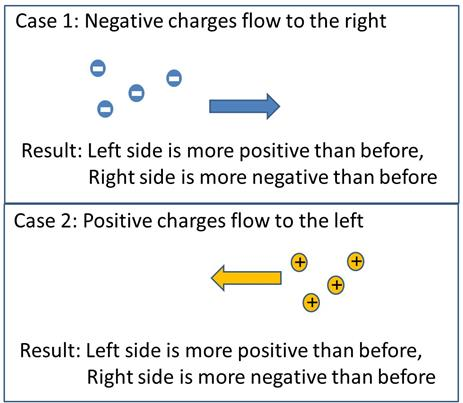
\includegraphics[width=3.8994in,height=3.3961in]{PH4CAU15}
\end{figure}

Worse yet, in biological things it \emph{is} positive ions that flow. So for biology a positive charge carrier is just fine.

Ben Franklin chose the direction we now use. He had a 50\% chance of making it easy for our electronics lab. But he got it backwards for us (but right for biology--and how many electronic things did Ben Franklin have anyway?). All this shows just how hard it is to deal with all these things we can't see or touch that we study in PH 220.

And even more importantly, in semiconductors--special electronic devices in all computers and in our Arduinos--it \emph{is} positive charge that flows. In many electrochemical reactions \emph{both} positive and negative charges flow. So Mr. Franklin was not really so very wrong. We will stick with the convention that \textbf{the current direction is the direction that positive charges would flow regardless of the actual charge carrier motion.} If you are like me, this will seem a little backwards, but we all get used to it.

But what makes the electrons or positive charges want to flow in the first place? We know the answer to this from earlier in this lab reading. It is potential energy. When we connect a metal wire to the terminals of a battery we know that the charges in the metal wire ends will experience a difference in potential energy. The potential energy difference will set up an electric field inside the conductor. 

\begin{figure}[h!]
	\centering
    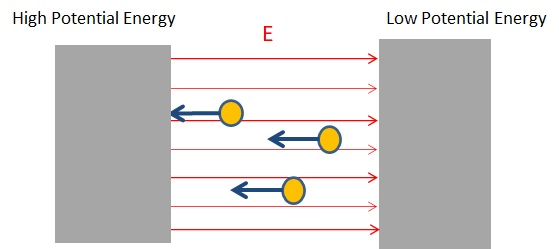
\includegraphics[width=4.2832in,height=1.53in]{PH4CAU16}
\end{figure}

This field makes the free charges move! It causes a force on the little electrons. We won't have to measure any fields in our lab today, but you should know they are there. The important thing is to realize that voltages produce currents. And the amount of current is proportional to the amount of
voltage. This is just Ohm's law! 

\begin{equation*}
	\Delta V=IR
\end{equation*}

The constant of proportionality is related to how much friction there is for the charges in the wire.

\begin{equation*}
	I=\frac{1}{R}\Delta V
\end{equation*}

It is just the resistance, $R$.\ 

\subsection{Knowing the Physics, Design the new instrument}

Now that we understand electrical current, we have some hope of figuring out how to build an instrument to measure that electrical current. From what we learned, consider adding in an additional small resistor in our circuit. If we take a small resistance, one that is small compared to all the other resistances in the circuit, and we put it in the circuit it will slow down the current, but not by very much. If the resistance is small enough, we won't even notice the change. Then if we measure the voltage across that small resistor with a voltmeter, we could mathematically calculate how much current we have. Notice that this instrument design has two parts. The first is adding some new hardware to our voltmeter (a resistor) and the second is adding in some calculation to get our voltmeter reading converted into current. Here is our equation for the calculation

\begin{equation*}
I=\frac{1}{R}\Delta V
\end{equation*}

And let's give this new additional small resistor a name. Let's call it the ``shunt resistor.''

\begin{equation*}
	I=\frac{\Delta V_{meter}}{R_{shunt}}
\end{equation*}

Today we will have to do the calculation part by hand. In future labs, we would carefully plan for this calculation in our Arduino sketch code.

\begin{figure}[h!]
	\centering
    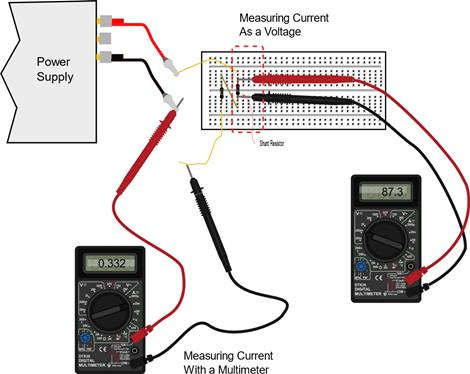
\includegraphics[width=4.9156in,height=3.9176in]{PH4CAU17}
\end{figure}

When we are done wiring our new instrument, we will have done something really cool. We have turned our current measurement into a voltage measurement plus a calculation. We measured something new in terms of a measurement we already knew how to make. We will generally try to do this for any type of
measurement. That is because we are very good at measuring voltage, and not so good at measuring other things electronically.

\subsection{Testing the new instrument}

We will need a way to test how good our new instrument works. And fortunately we know our multimeters can also measure current. So we can build our new instrument an compare it to the measurement made by a multimeter. This test of a new instrument is an important part of designing a new instrument!

\begin{equation*}
	\unit{A}=\frac{\unit{V}}{\unit{\Omega}}
\end{equation*}

Recall that to use an ammeter (the new instrument we build, or the one in our multimeter), you must break the electric circuit by disconnecting a wire. Then you replace that wire with the ammeter. Notice that in the diagram below that the bottom wire is now broken. 

\begin{figure}[h!]
	\centering
     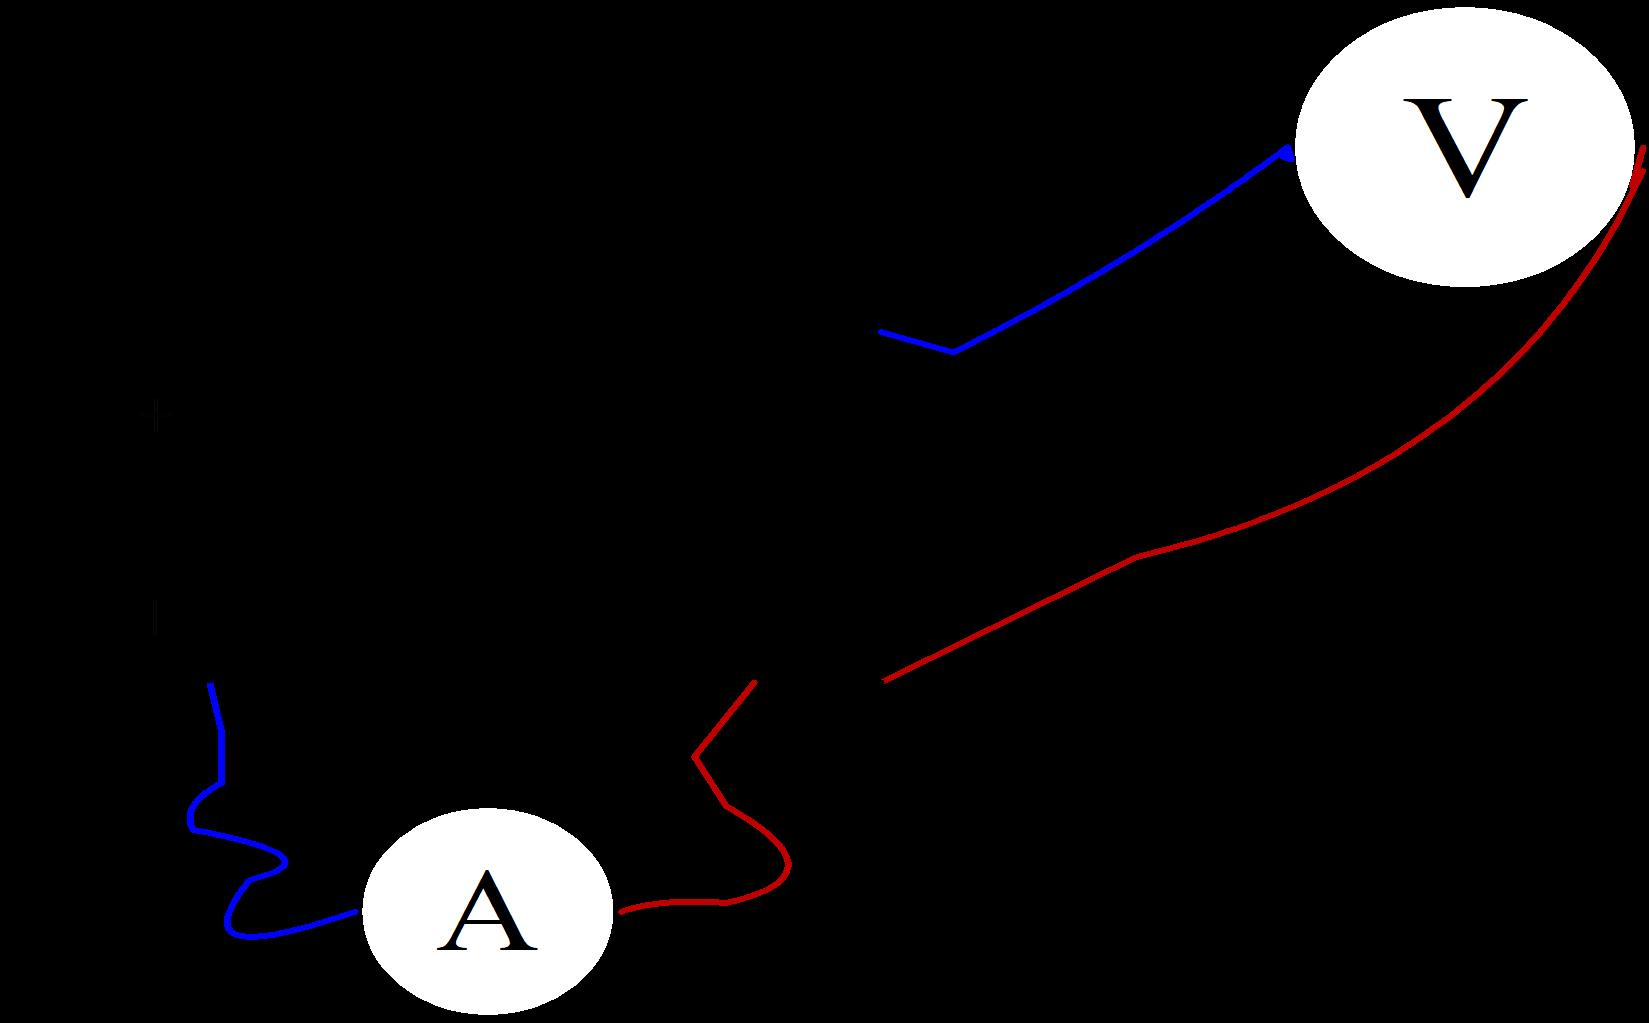
\includegraphics[width=1.9372in,height=1.471in]{PH4CAU18}
\end{figure}

Where a wire was, I have drawn an ammeter. The current must flow through the ammeter for us to measure it.

\begin{figure}[h!]
	\centering
    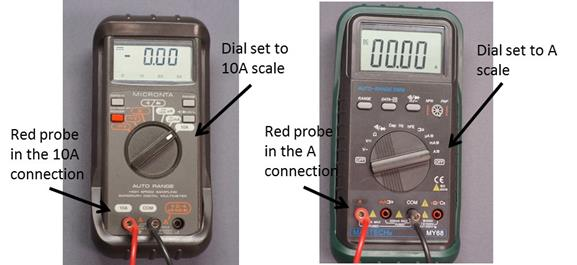
\includegraphics[width=4.858in,height=2.2423in]{PH4CAU19}
\end{figure} 

Remember, to use our multimeters to measure current, we must turn the dial to the $10\unit{A}$ setting AND move the red probe to the $10\unit{A}$ connector. Failure to do this may result in the fuse blowing. Our meter does not warn you that it lost a fuse, it just pays you back by giving really wrong answers. You should be careful to connect it right, and be sure it is working (that someone else has not blown the fuse before you). Since we have different kinds of multimeters, a
second is pictured to the right. For this type of meter, put the red lead in the connector marked $A$ and turn the dial to the $A$ setting. If the currents you are measuring are very small, you might have to switch settings once again. Tiny currents can be measured by moving the dial to the $\unit{mA}$ setting AND changing the red probe to the $\unit{mA}$ connector.

\begin{figure}[h!]
	\centering
    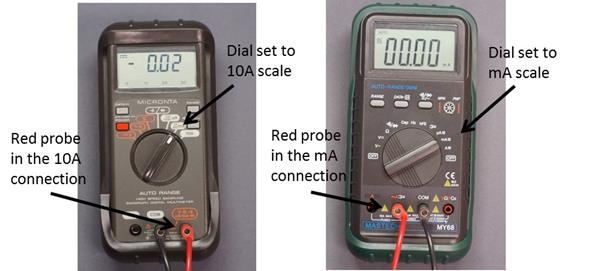
\includegraphics[width=4.9769in,height=2.2928in]{PH4CAU1A}
\end{figure}

Our multimeters really measure current in much the same way we are talking about for our new Arduino ammeter. They have a series of shunt resistors inside of them. When we choose a current measurement setting we are choosing a shunt resistor to put in the circuit (inside the meter, but the meter is in the circuit). Then the voltmeter will measure the voltage across that resistor and use that voltage to calculate the current.

If we create the current meter ourselves, we have to know the resistance that we used! That allows us to use the voltage meter to calculate the current,

\begin{equation*}
	I=\frac{\Delta V_{meter}}{R_{shunt}}
\end{equation*}

but our multimeters are programed to know their own shunt resistances and to do this calculation for us.

If you have time (and some won't) in today's lab, we will build the new Arduino instrument to measure current , and we will test it with a multimeter set in ammeter mode. We will put both in the circuit at the same time (see figure \ref{New Instrument and Test} in the assignment section below) so we get readings from both. Then we can compare and see how well our new instrument works!

\section{Calculating uncertainty, a review}

That is all the new material for today's lab. But I wanted to remind you of
something you already know.

Back in PH150 you should have gotten a good deal of experience in making
measurements. We will be going back to experimentation soon, and we will
need to remember what we learned in PH150 to take the measurements so that
we can interpret our experimental results. You will remember that every
measurement has an uncertainty. We have to estimate that uncertainty. It
turns out that our voltage measurement schemes will introduce a new source
of uncertainty! And we will have to include this in our uncertainty
calculations. We will take that on next lab, but in this lab let's review
how to calculate uncertainties (If you took our PH150 recently, you can skip this section!).

This is a ``review.'' How much of a ``review'' it is may depend on where and when you took PH150 or its equivalent. If you are a chemist, you will note that our treatment of uncertainty goes beyond what you learned in Quantitative Analysis. Let's start by reviewing what a derivative is.

For our purposes, a derivative is a slope of a line. You should recognize the equation of a straight line as

\begin{equation*}
	y=mx+b
\end{equation*}

The slope $m$ can be written as 

\begin{equation*}
	m=\frac{dy}{dx}
\end{equation*}

This is nothing magic (or new). It is just a strange way to write $m.$ With the slope written this way, the equation of the line could be written as 

\begin{equation*}
	y=\frac{dy}{dx}x+b
\end{equation*}

But why $dy/dx$? Think of how we find a slope of a line. Back in junior high
school we called the slope the ``rise over run.'' That is, the change in $y$-value divided by the
change in the $x$-value.

\begin{equation*}
	m=\frac{y_{2}-y_{1}}{x_{2}-x_{1}}
\end{equation*}

In physics, we write the change in a variable using the Greek letter delta, $\Delta .$ So we could write the slope as

\begin{equation*}
	m=\frac{y_{2}-y_{1}}{x_{2}-x_{1}}=\frac{\Delta y}{\Delta x}
\end{equation*}

Just to jog your memory, let me write out $\Delta y$

\begin{equation*}
	\Delta y=y_{2}-y_{1}
\end{equation*}

and $\Delta x.$ 

\begin{equation*}
	\Delta x=x_{2}-x_{1}
\end{equation*}

So our straight line equation should be written 

\begin{equation*}
	y=\frac{\Delta y}{\Delta x}x+b
\end{equation*}

but if we take $\Delta x$ to be very, very small it is customary to write the $\Delta x$ as just $dx$ (I guess a ``$d$'' is smaller than a ``$\Delta $'' ). If this is not familiar from Math 112, is should be by now from PH121.

In PH121 you learned that the velocity is the slope of the plot of $x$ vs. $t,$ for example, 

\begin{equation*}
	y=\frac{1}{2}\frac{\unit{m}}{\unit{s}}t+1\unit{m}
\end{equation*}

is an equation giving the $y$ position of an object as a function of time. Note that it is a straight line on a $y$ vs. $t$ plot. 

\begin{figure}[h!]
	\centering
    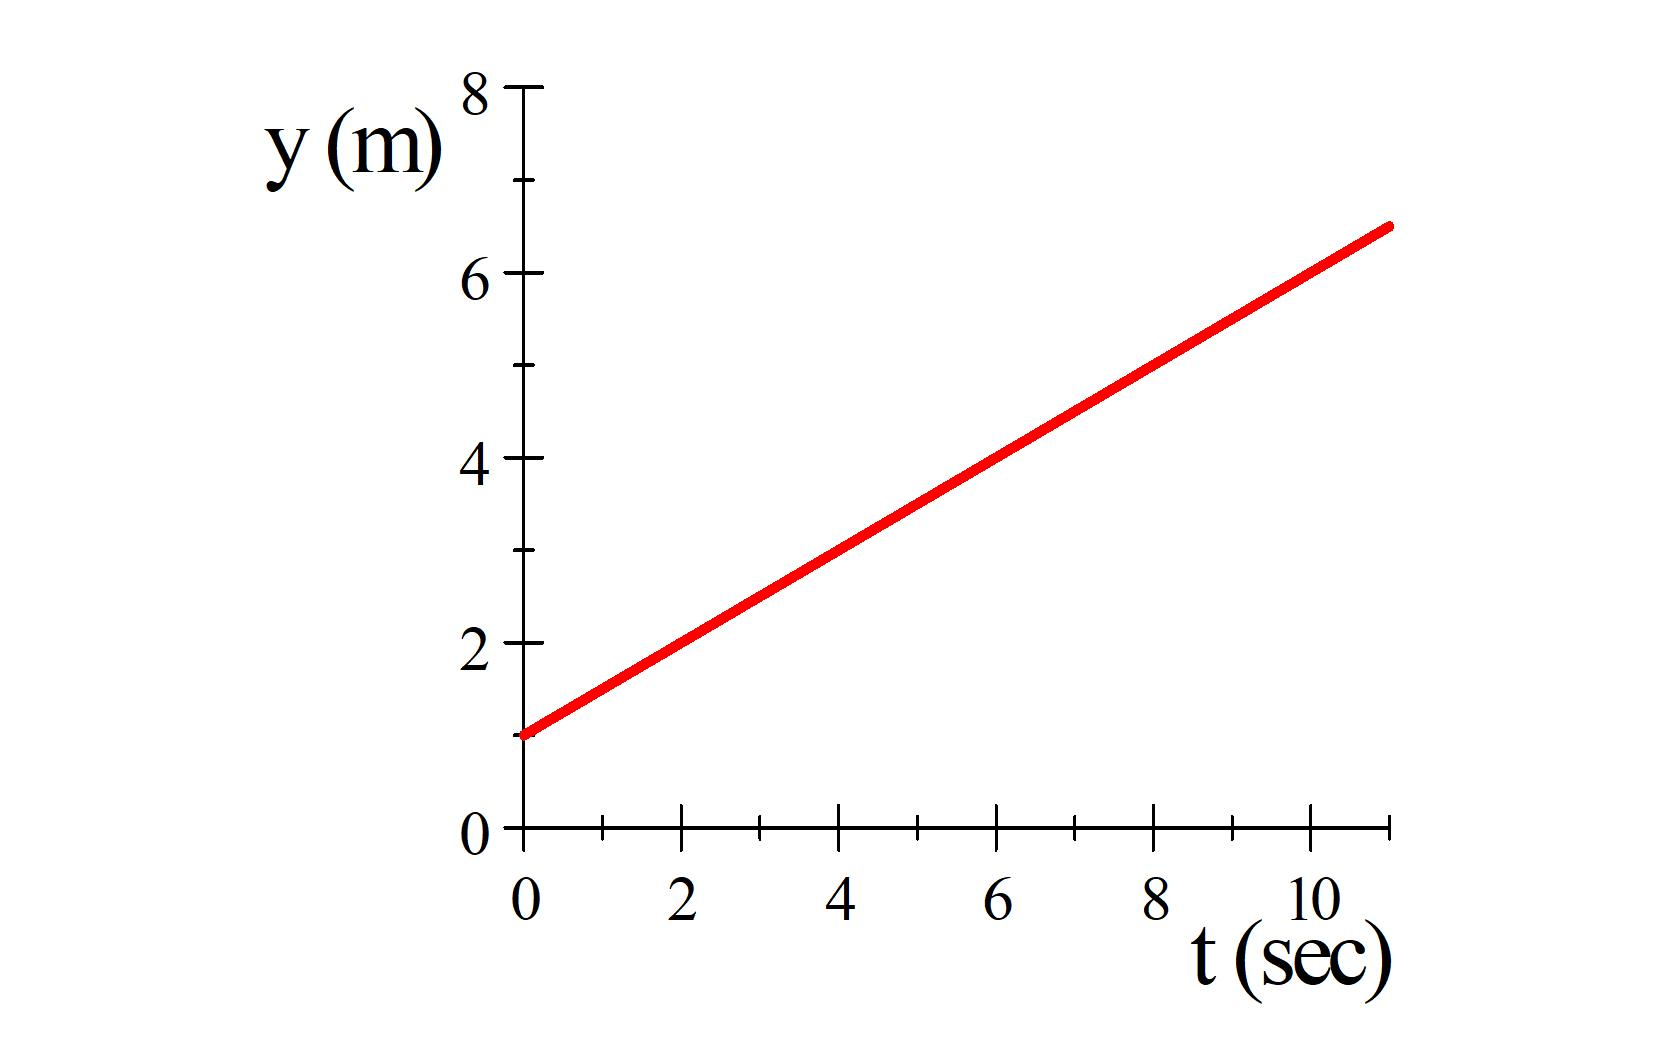
\includegraphics[width=3.3in,height=1.68in]{PH4CAU1B}
\end{figure}

The slope of the line is 

\begin{equation*}
	\frac{dy}{dt}=\frac{1\unit{m}}{2\unit{s}}
\end{equation*}

We can verify that this works by looking at the plot and noting that for every two units of time, we go up one position unit. The slope is $1/2\frac{\unit{m}}{\unit{s}}.$

But not all curves are straight lines. What do we do with curves that, well, curve?

One idea is that we could split up the curve into little line segments, each with its own slope. We can think of $dy/dt$ as an instantaneous slope, a slope of one of the tiny line segments that make up our curve. This is the sort of speed measurement that your speedometer gives. The speed might be different a short time later. But right now the speed is, say, $0.5\unit{m}/ \unit{s}.$

\begin{figure}[h!]
	\centering
    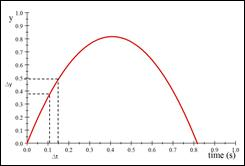
\includegraphics[width=2.8in,height=1.7in]{PH4CAU1C}
\end{figure}

Really, in defining an instantaneous slope we have assumed that the slope near our point on the
curve is essentially a straight line if $\Delta t$ is small enough.

We can use this idea to interpret our error calculations. Suppose I\ throw a ball in the air with a initial speed of $4\unit{m}/\unit{s}$ straight up starting from $y_{o}=0$. From PH121 you have learned that the equation for predicting how high the ball will go is 

\begin{equation*}
	y=y_{o}+v_{o}t+\frac{1}{2}at^{2}
\end{equation*}

It says that starting at $y_{o}$ the ball will go higher depending on the initial velocity, $v_{o},$ and the acceleration, $a.$ That makes sense.

At a time, $t,$ the ball should be at 

\begin{equation*}
	y=0+4\frac{\unit{m}}{\unit{s}}t-\frac{1}{2}\left( 9.8\frac{\unit{m}}{\unit{s}^{2}}\right) t^{2}
\end{equation*}

where $a=-9.8\frac{\unit{m}}{\unit{s}^{2}}$ is the acceleration due to gravity. So, knowing this, I could predict how high the ball would go if I pick a particular time, say, $0.15\unit{s}.$ The result should be

\begin{eqnarray*}
	y &=&0+4\frac{\unit{m}}{\unit{s}}\left( 0.15\unit{s}\right) -\frac{1}{2} \left( 9.8\frac{\unit{m}}{\unit{s}^{2}}\right) \left( 0.15\unit{s}\right) ^{2} \\
      &=&0.489\,75\unit{m}
\end{eqnarray*}

This is shown in the next figure with a black line. Solving the equation for $y$ is equivalent to drawing a line up to the curve, then from our spot on the curve over to the $y$-axis to find the position.

\begin{figure}[h!]
	\centering
    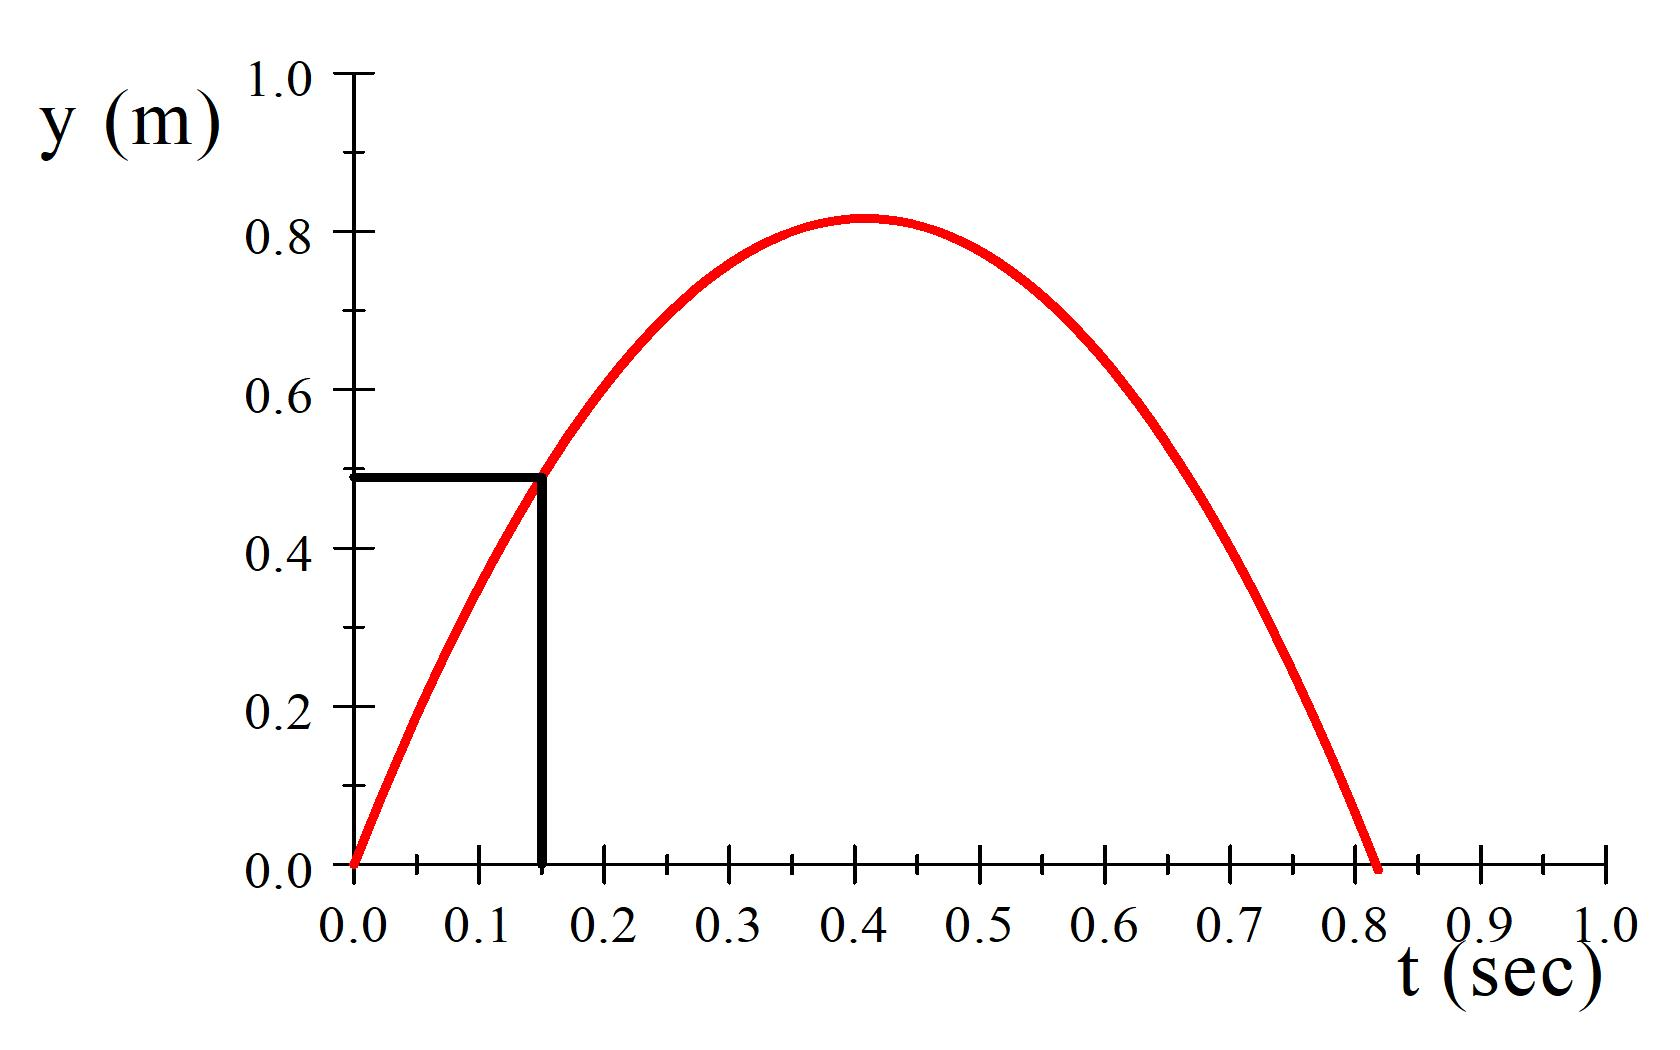
\includegraphics[width=3.3434in,height=2.2295in]{PH4CAU1D}
\end{figure}

For our case, we plot a line upward from $0.15\unit{s}$ to the curve, and then plot a horizontal line from the intersection to the $y$-axis. We can see that we get $4.9\unit{m}.$ Suppose I try to verify this by taking a picture of the ball in flight at $0.015\unit{s},$ but my stop watch is only
good to $\pm 0.005$ seconds. I try to take the picture when the watch is at $0.015\unit{s},$ but I might have taken the picture at $0.01\unit{s}$ or at $0.02\unit{s}$ or anywhere in between. My time has some uncertainty. What does the uncertainty in my stop watch time mean for the uncertainty in my $y$ value?

We can get a good approximation by graphically drawing vertical lines up from $t_{\min }$ and $t_{\max }$ to the curve, and then extending horizontal lines from the intersections to the $y$-axis. This gives us a $y_{\min }$ and $y_{\max }.$ Our actual height could be anywhere in between these. This is a way to view our uncertainty in $y.$

\begin{figure}[h!]
	\centering
    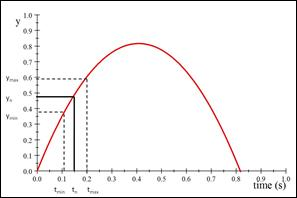
\includegraphics[width=4.1658in,height=2.7769in]{PH4CAU1E}
\end{figure}

We can use this idea to find a general way to calculate uncertainties. We could define $\Delta t=t_{\max }-t_{\min }$. If our $\Delta t$ is small enough (so we can write it just $dt$), the curve is essentially a straight line in the region between $t_{\min }$ and $t_{\max }.$ So if we knew the
slope of that line (the derivative $dy/dt$) we could easily figure out the $y_{\max }$ and $y_{\min }$ points to get our uncertainty range, at least if we stay near our $t_{n}$ part of the curve. Recall that our uncertainty in $y$ is about

\begin{equation*}
	\delta y=\frac{y_{\max }-y_{\min }}{2}=\frac{\Delta y}{2}
\end{equation*}

Remembering that 

\begin{equation*}
	y=\frac{dy}{dt}t+b
\end{equation*}

then 
\begin{eqnarray*}
	\Delta y &=&y_{\max }-y_{\min } \\
			 &=&\frac{dy}{dt}t_{\max }+b-\frac{dy}{dt}t_{\min }-b \\
             &=&\frac{dy}{dt}\Delta t
\end{eqnarray*}

From PH150, you will recognize this as almost the uncertainty in a function of one variable! But even if you don't recognize it, we can show that this is true using our definition of $\delta y$ above. The quantity $\Delta t$ is 

\begin{equation*}
	\Delta t=t_{\max }-t_{\min }
\end{equation*}

so our uncertainty in $t$ would be 

\begin{equation*}
	\delta t=\frac{t_{\max }-t_{\min }}{2}=\frac{\Delta t}{2}
\end{equation*}

then 

\begin{eqnarray*}
	\delta y &=&\frac{y_{\max }-y_{\min }}{2} \\
             &=&\frac{1}{2}\frac{dy}{dt}\Delta t \\
             &=&\frac{dy}{dt}\frac{\Delta t}{2} \\
             &=&\frac{dy}{dt}\delta t
\end{eqnarray*}

so

\begin{equation*}
   \delta y=\frac{dy}{dt}\delta t
\end{equation*}

So our uncertainty in $y$ is just the slope at our point on the curve multiplied by our uncertainty in $t.$

But what if we have more than one variable? Say, we have a function $y(x,z),$ we essentially have a two dimensional slope. Think of a hill, you can go down a hill in more than one direction. So we need slope parts for each direction we can go.

\begin{figure}[h!]
	\centering
    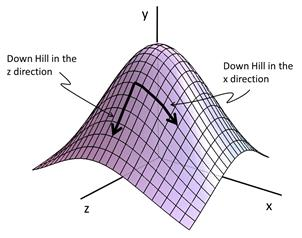
\includegraphics[width=2.3495in,height=1.8133in]{PH4CAU1F}
\end{figure}

\begin{equation*}
   \Delta y=\frac{dy}{dx}x\hat{\imath}+\frac{dy}{dz}z\hat{k}
\end{equation*}

But there is a fix we need to make to this equation that you won't learn for several math classes to come. We want to have a slope in the $x$ and $z$ direction, but we want the slopes to be independent. Think back in PH121 when we did two dimensional motion problems, we split the problem into components. We want to do this for our two dimensional uncertainty! The notation for this is

\begin{equation*}
	\Delta y_{x}=\frac{\partial y}{\partial x}x
\end{equation*}

\begin{equation*}
	\Delta y_{z}=\frac{\partial y}{\partial z}z
\end{equation*}

where 

\begin{equation*}
	\frac{\partial y}{\partial x}
\end{equation*}

means the component of the slope \textbf{just} in the $x$ direction. We take a derivative of the function $y,$ but assume only $x$ is a variable (treat $z$ and all $z$ terms with no $x^{\prime }s$ as constants). This lets us separate the $x$ and $z$ parts. A special, one variable derivative like $\partial y/\partial x$ is called a \emph{partial derivative} because you only take one dimension of the derivative at a time. So, if we wish to find the error in some general function $z\left( x,y\right) $ the error is given by
 
\begin{equation*}
	\delta y=\sqrt{\left( \frac{\partial y}{\partial x}\right) ^{2}\delta x^{2}+\left( \frac{\partial y}{\partial z}\right) ^{2}\delta z^{2}}
\end{equation*}

This looks a lot like our slope equation. What we are doing is to assuming the function $y\left( x,z\right) $ is flat in a small region around the point we are studying. then the function has a slope $\partial y/\partial x$ in the $x$-direction, and $\partial y/\partial z$ in the $y$-direction. Each term like 

\begin{equation*}
	\left( \frac{\partial y}{\partial x}\right) \delta x
\end{equation*}

gives how far off we could be in that direction (the $x$-direction in this case). Remember that we have assumed that $y\left( x,z\right) $ is essentially flat near our point of interest. The square root may be something of a mystery, but remember what you have learned about adding vectors in PH121. We add components of a vector to find the magnitude like this
 
\begin{equation*}
	V=\sqrt{V_{x}^{2}+V_{y}^{2}}
\end{equation*}

This comes from the Pythagorean theorem. The $x$ and $y$ parts of the vector form two sides of a triangle. We want the remaining side. So we use the Pythagorean theorem to find the length of the remaining side.

We are doing the same for our small uncertainty lengths. We are just adding the $x$ and the $y$ components of the error. We could write our error formula for the general case of a function $f$, that depends on $N$ different variables. 

\begin{equation*}
	\delta f=\sqrt{\sum_{i=1}^{N}\left( \frac{\partial f}{\partial x_{i}}\right)^{2}\delta x_{i}^{2}}
\end{equation*}

We will use this formula a lot, so make sure you understand what it means (ask your instructor for help if it is not clear).

\subsection{How do we find the slope?}

But now we have an equation in terms of slope written as $\partial y/\partial x$ or $\partial y/\partial z$, but how would we ever find these slopes? Your calculus class has or will teach you how to take a derivative. They might not have yet taught you how to take this type of derivative. The symbol $\partial $ means that our derivatives are ``partial'' derivatives. This means that we assume all the variables other than the one that shows up in the derivative symbol are constants for our derivative.

Let's take an example. What is the slope of the function $y=5zx^{3}?$ if we calculate the slope only going in the $x$-direction (that is, if we take a partial derivative with respect to $x$) we get

\begin{equation*}
   \frac{\partial }{\partial x}\left( 5zx^{3}\right) =5z\left( 3\right) x^{3-1}=15zx^{2}
\end{equation*}

notice that we treated $z$ as a constant! That is what we mean when we user the symbol $\partial $ and when we say \textquotedblleft partial derivative.\textquotedblright\ Let's try another. How about finding the slope of $f=7yx^{2}-2x+z$ with respect to the $x$-direction.

\begin{equation*}
   \frac{\partial }{\partial x}\left( 7yx^{2}-2x+z\right) =7y\left( 2\right)x^{1}-2(1)x^{0}+z\left( 0\right)
\end{equation*}

The last term illustrates that the slope of a constant is zero, and as we go just in the $x$-direction, $z$ is constant. That makes sense. So the change in $f$ just due to the last term $(z)$ should be zero. We also remember $x^{0}=1.$ So we are left with 

\begin{equation*}
	\frac{\partial }{\partial x}\left( 7yx^{2}-2x+z\right) =14yx-2
\end{equation*}

We could also find 

\begin{equation*}
	\frac{\partial }{\partial y}\left( 7yx^{2}-2x+z\right) =7x^{2}
\end{equation*}

and

\begin{equation*}
	\frac{\partial }{\partial z}\left( 7yx^{2}-2x+z\right) =1
\end{equation*}

In our equation for calculating uncertainties, we want to find the uncertainty in each dimension (for each variable) and to add these uncertainties like components of vectors, so this partial derivative is just what we want, the slope of our function in just one direction.

\subsubsection{Tie to statistics}

Back in PH150 you should have learned that for experiments where we repeat the same experiment over and over again, our outcome can be given by the mean value an our uncertainty can be given by the standard deviation. We need to tie our statistical ideas into what we have learned about error propagation. Lets go back to our function $f\left( x,z\right) $ the error is given by 

\begin{equation*}
	\delta f=\sqrt{\left( \frac{\partial f}{\partial x}\right) ^{2}\delta x^{2}+\left( \frac{\partial f}{\partial z}\right) ^{2}\delta z^{2}}
\end{equation*}

but now we know we could express this in terms of standard deviations (provided you don't need to ensure every bit of your data are within your uncertainty range). We can write our uncertainties as 

\begin{equation*}
	\sigma _{f}=\sqrt{\left( \frac{\partial f}{\partial x}\right) ^{2}\sigma_{x}^{2}+\left( \frac{\partial f}{\partial z}\right) ^{2}\sigma _{z}^{2}}
\end{equation*}

So one way to get an estimate of uncertainty like $\delta x$ or $\delta z$ above is to make many measurements, and use the standard deviation $\sigma_{x}$ as an estimate for $\delta x$ and $\sigma _{z}$ for $\delta z.$ This is usually not too far off (we will refine this analysis in PH336 for those lucky enough to take the course).

We can use connection between $\delta x$ and $\sigma _{x}$ to show that the standard deviation of the mean (the best estimate of our uncertainty) is given by

\begin{equation*}
	\sigma _{\bar{x}}=\frac{\sigma _{x}}{\sqrt{N}}
\end{equation*}

(a result you should have learned back in PH150). Think of calculating a mean value

\begin{equation*}
	\bar{x}=\frac{x_{1}+x_{2}+\cdots x_{N}}{N}
\end{equation*}

We can find the uncertainty in this function $\sigma _{\bar{x}}$

\begin{equation*}
	\sigma _{\bar{x}}=\sqrt{\left( \frac{\partial \bar{x}}{\partial x_{1}} \right) ^{2}\sigma _{x_{1}}^{2}+\left( \frac{\partial \bar{x}}{\partial x_{2}}\right) ^{2}\sigma _{x_{2}}^{2}+\cdots +\left( \frac{\partial \bar{x}}{\partial x_{N}}\right) ^{2}\sigma _{x_{N}}^{2}}
\end{equation*}

You see we just take the partial derivative of our function $\bar{x}$ with respect to each of the variables $x_{i}$ and multiply by the uncertainty in that variable written now as a standard deviation $\sigma _{i}.$

For this special case, all of the $x_{i}$ are the same (we are measuring the same value over and over in taking an average) and all of the $\sigma _{i}$ are the same so we just have

\begin{equation*}
	\sigma _{\bar{x}}=\sqrt{N\left( \frac{\partial \bar{x}}{\partial x_{1}} \right) ^{2}\sigma _{x_{1}}^{2}}
\end{equation*}

and we can take the derivative using our rule. Only $x_{1}$ is a variable, so we can write the average $\bar{x}$ as 

\begin{equation*}
	\bar{x}=\frac{x_{1}}{N}+\frac{x_{2}+\cdots x_{N}}{N}
\end{equation*}

This is a polynomial! The first term is $\frac{1}{N}x_{1}$ and the whole second term is a constant if we take a partial derivative with respect to $x_{1}$. The derivative is 

\begin{eqnarray*}
	\frac{\partial \bar{x}}{\partial x_{1}} &=&\frac{\partial }{\partial x_{1}}\left( \frac{x_{1}}{N}+\frac{x_{2}+\cdots x_{N}}{N}\right) \\
                                            &=&\frac{1}{N}x_{1}^{0}+0 \\
                                            &=&\frac{1}{N}
\end{eqnarray*}
so our statistical error function is just 

\begin{eqnarray*}
	\sigma _{\bar{x}} &=&\sqrt{N\left( \frac{1}{N}\right) ^{2}\sigma _{x_{1}}^{2}} \\
                      &=&\sqrt{\frac{\sigma _{x_{1}}^{2}}{N}} \\
                      &=&\frac{\sigma _{x_{1}}}{\sqrt{N}}
\end{eqnarray*}

or, since all the $\sigma _{x_{i}}$ are the same, we can just write this as 

\begin{equation*}
	\sigma _{\bar{x}}=\frac{\sigma _{x}}{\sqrt{N}}
\end{equation*}

Notice that in this example we had many $x_{i}$ and that to find the uncertainty we just extended our equation from two variables

\begin{equation*}
	\sigma _{f}=\sqrt{\left( \frac{\partial f}{\partial x}\right) ^{2}\sigma_{x}^{2}+\left( \frac{\partial f}{\partial z}\right) ^{2}\sigma _{z}^{2}}
\end{equation*}

to $N$ variables

\begin{equation*}
	\sigma _{f}=\sqrt{\sum_{i=1}^{N}\left( \frac{\partial f}{\partial x_{i}}\right) ^{2}\sigma _{i}^{2}}
\end{equation*}

In this special case, we were trying to show a special result, but we can do this for any function with any number of variables. If your function is complicated, you just need to take more partial derivative terms under the square root.

I'm sure you remembered all of that from PH150. But now it is time to move on to today's lab assignment.
\vfill
\pagebreak
\section{Practice Measurements}
Here are some measurements to try with the instruments we learned about in this reading.

\subsection{Use a Multimeter}

\begin{enumerate}
\item Measure the voltage of a D-Cell battery with a voltmeter. Report the value you get from the measurement and the uncertainty.

\item Set up the circuit described in section (\ref{Voltage Measurement with Meter}). The figure is repeated below. Measure the voltage with a multimeter. \textbf{The indicator on the power supply is not very accurate}, but it can serve as a check to see if we are way off. So compare the power
supply voltage indicator to the meter indicator. Are they the same (you should think of the uncertainty in both meters and answer using the uncertainties)

\begin{figure}[h!]
	\centering
    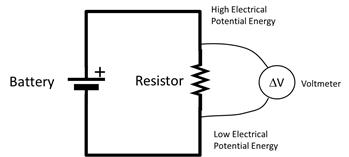
\includegraphics[width=4in,height=2in]{PH4CAU1G}  
\end{figure}

\item Modify your circuit described in section (\ref{Voltage Measurement with Meter}) and change the settings of your multimeter so that you measure the current in the circuit. Compare your ammeter measurement to the current shown on the power supply indicator.
\end{enumerate}

\subsection{Use an Oscilloscope}

\begin{enumerate}
\item Predict what you will see on an oscilloscope if you measure the voltage of a D-Cell battery. Make sure your lab table agrees on your prediction before you go on.

\item Use the oscilloscope to measure the voltage of a D-Cell battery.

\item Practice interpreting oscilloscope screens

\begin{enumerate}
\item Figure out what the markings on the Oscilloscope screen mean.

\item Figure out what the voltage scale is and how to change it

\item Figure out what the time scale is and how to change it
\end{enumerate}

\item Generate a sinusoidal signal using the stand alone Signal Generator.

\item Measure and display this signal using the stand alone digital
oscilloscope.

\item Report the amplitude and the frequency (and their uncertainties) of
the measured signal and compare to the signal generator settings.
\end{enumerate}

\subsection{Build a new instrument from an old instrument}

\begin{enumerate}
\item IF\ THERE\ IS\ TIME, choose a resistor in the $20\unit{k\Omega}$ range (say, from about $10\unit{k\Omega}$ to about $30\unit{k\Omega}$). Choose a shunt resistor in the $200\unit{\Omega}$ range. Then set up the circuit to measure a current. 

\begin{figure}[h!]
	\centering
    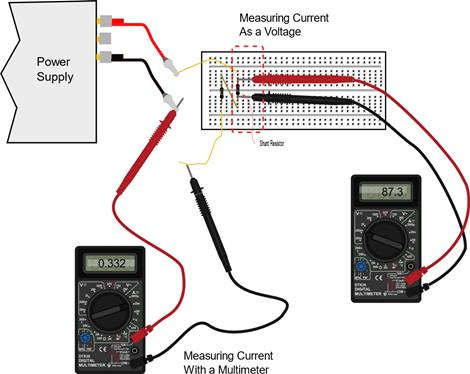
\includegraphics[width=3.8744in,height=3.0874in]{PH4CAU1H}
    \label{New Instrument and Test}
\end{figure}

Use an additional multimeter set to measure current to check our
voltage-current measurement. Calculate a percent difference to see how well
this worked.
\end{enumerate}


\vspace*{\fill}
\pagebreak